\chapter{理想流体：欧拉与伯努利}\label{ch:b2:euler-bernoulli}

把一张纸的一边捏住，对着它的上表面吹气，纸便会抬起。打开
淋浴的水龙头，浴帘便会向内飘。飞机机翼能托起三百吨，
是因为气流经过上表面的速度比下表面大。这三种现象
说的是同一件事：\emph{流体流动越快，压强越小}。本章
在最简单的模型中写\omterm{prop:b2:euler-bernoulli:torricelli}{出流}体微团的牛顿第二定律，
所用模型为最简单的\emph{理想}流体——只承受压强而无摩擦的流体，
由此导出伯努利定理，即\omterm{def:b2:fluid-kinematics:euler}{流线}上的能量平衡，
其应用从管道中的流量计，
一直到飞机的
空速表。

\section{欧拉方程}

\begin{proposition}[流体微团所受的压力]\label{prop:b2:euler-bernoulli:pressure}
\index{压力（体积密度）}
周围流体作用于体积为
$\dd\tau$ 的微团上的压力的合力为
\[
\dd\vect F_P = -\operatorname{\vect{grad}}P\,\dd\tau :
\]
压强相当于一种体积力，其密度为 $-\operatorname{\vect{grad}}P$，
方向由高压指向低压。
\end{proposition}

\begin{proof}
在\cref{thm:b2:fluid-kinematics:continuity}中的小六面体上，位于
$x$ 与 $x + \dd x$ 处的面分别受到 $+P(x)\dd y\dd z$ 与 $-P(x + \dd x)\dd y\dd z$ 的压力，
沿 $x$ 方向合力为 $-\partial_xP\,\dd x\dd y\dd z$；沿 $y$、$z$ 方向同理。
\end{proof}

\begin{definition}[理想流体]\label{def:b2:euler-bernoulli:perfect}
\index{理想流体}
若流体中相邻微团之间唯一的接触力是压力，则称该流体为\emph{理想流体}。
压力垂直于每一个面，不存在切向（粘性）应力。这是一种理想化模型，
正如下一章所说明的，它在远离壁面且雷诺数很大时成立：
管道中远离管壁的水，
机翼周围薄边界层之外的空气，
海面上的波浪。
\end{definition}

\begin{theorem}[欧拉方程]\label{thm:b2:euler-bernoulli:euler}
\index{欧拉方程}
在伽利略参考系中，密度为 $\rho$ 的\omterm{def:b2:euler-bernoulli:perfect}{理想流体}，
受重力作用，在每一点都满足
\[
\rho\Bigl(\frac{\partial\vect v}{\partial t} + (\vect v\cdot\operatorname{\vect{grad}})
\vect v\Bigr) = -\operatorname{\vect{grad}}P + \rho\vect g ,
\]
若还存在其他体积力密度 $\vect f_v$（如电场力，或
非伽利略参考系中的惯性力），则应在右端加上该项。静止时，上式化为
本科一年级分册中的流体静力学定律
$\operatorname{\vect{grad}}P = \rho\vect g$。
\end{theorem}

\begin{proof}
对质量为 $\rho\,\dd\tau$ 的流体微团应用牛顿第二定律：其
加速度为物质导数
（见\cref{thm:b2:fluid-kinematics:material}），所受的力为压力的合力
与重力 $\rho\vect g\,\dd\tau$；两边除以 $\dd\tau$ 即得。
\end{proof}

\begin{example}[加速运动的水箱]\label{ex:b2:euler-bernoulli:tank}
装在以 $\vect a$ 加速行驶的卡车上的水箱中，水在卡车参考系中静止；
在该参考系中，对惯性力 $-\rho\vect a$ 应用\omterm{thm:b2:euler-bernoulli:euler}{欧拉方程}，
得 $\operatorname{\vect{grad}}P = \rho(\vect g - \vect a)$：压强
沿“等效重力” $\vect g - \vect a$ 的方向增大，自由面
（等压面）与之垂直，并向后倾斜，
倾角为 $\arctan(a/g)$——当 $a = \qty{2}{m/s^2}$ 时为 \qty{11}{\degree}。在
以 $\Omega$ 旋转的水桶中，离心力 $\rho\Omega^2r\,\vect e_r$
给出 $P = P_0 + \tfrac12\rho\Omega^2r^2 - \rho gz$，自由面为
旋转抛物面 $z = \Omega^2r^2/2g$。
\end{example}

\begin{omfigure}
\begin{tikzpicture}[font=\small, x=1cm, y=1cm, >=Stealth]
  \begin{scope}
    \draw[thick, fill=omDef!10] (0,0) rectangle (1.8,1.4);
    \draw[omThm, very thick, ->] (-1.0,0.7) -- (-0.05,0.7) node[pos=0.2, above, font=\footnotesize] {$P(x)\,\dd S$};
    \draw[omThm, very thick, ->] (2.85,0.7) -- (1.85,0.7) node[pos=0.1, above, font=\footnotesize] {$P(x+\dd x)\,\dd S$};
    \draw[omThm, very thick, ->] (0.9,-1.0) -- (0.9,-0.05);
    \draw[omThm, very thick, ->] (0.9,2.4) -- (0.9,1.45);
    \node[font=\footnotesize] at (0.9,-1.4) {$\dd\vect F_P = -\operatorname{\vect{grad}}P\,\dd\tau$};
  \end{scope}
  \begin{scope}[xshift=6.0cm]
    \draw[thick] (-1.6,-0.2) -- (-1.6,1.6) (-1.6,-0.2) -- (1.6,-0.2) -- (1.6,1.6);
    \draw[omDef, thick, fill=omDef!15] (-1.6,1.4) -- (1.6,0.2) -- (1.6,-0.2) -- (-1.6,-0.2) -- cycle;
    \draw[->, very thick] (0,1.9) -- (0.45,1.9) node[right, font=\footnotesize] {$\vect a$};
    \draw[omThm, ->, thick] (0,0.5) -- (0,-0.7) node[right, font=\footnotesize] {$\vect g$};
    \draw[omProp, ->, thick] (0,0.5) -- (-0.45,-0.7) node[left, font=\footnotesize] {$\vect g - \vect a$};
    \node[font=\footnotesize] at (0,-1.4) {加速水箱：液面 $\perp \vect g - \vect a$};
  \end{scope}
  \begin{scope}[xshift=11.2cm]
    \draw[thick] (-1.4,-0.2) -- (-1.4,1.8) (-1.4,-0.2) -- (1.4,-0.2) -- (1.4,1.8);
    \draw[omDef, thick, fill=omDef!15, domain=-1.4:1.4, samples=40] plot (\x,{0.35+0.6*\x*\x}) -- (1.4,-0.2) -- (-1.4,-0.2) -- cycle;
    \draw[dashed] (0,-0.5) -- (0,2.1);
    \draw[->] (-0.3,2.0) arc[start angle=150, end angle=30, radius=0.35] node[right, font=\footnotesize] {$\Omega$};
    \node[font=\footnotesize] at (0,-1.4) {旋转水桶：$z = \Omega^2r^2/2g$};
  \end{scope}
\end{tikzpicture}

{\small 左：当 $P$ 变化时，流体小六面体各面上的压力不能相互抵消，
其合力为单位体积的 $-\operatorname{\vect{grad}}P$。
中、右：两种静止于加速参考系中的流体，
自由面处处与
等效重力垂直。}
\end{omfigure}

\section{伯努利定理}

\begin{theorem}[伯努利]\label{thm:b2:euler-bernoulli:bernoulli}
\index{伯努利定理}\index{滞止压强}\index{动压}
对于密度均匀的\emph{理想}、\emph{不可压缩}流体作
\emph{定常}流动，在重力均匀的伽利略参考系中，量
\[
P + \tfrac12\rho v^2 + \rho gz
\]
该量沿每条\emph{\omterm{def:b2:fluid-kinematics:euler}{流线}}保持不变。若流动还是
\emph{无旋}的，则该量在整个流体中处处相同。
项 $\tfrac12\rho v^2$ 称为\emph{\omterm{thm:b2:euler-bernoulli:bernoulli}{动压}}；$P + \tfrac12\rho v^2$
为\emph{\omterm{thm:b2:euler-bernoulli:bernoulli}{滞止压强}}，即流体若沿其\omterm{def:b2:fluid-kinematics:euler}{流线}被带至静止时
所能达到的压强。
\end{theorem}

\begin{proof}
对定常\omterm{thm:b2:euler-bernoulli:euler}{欧拉方程}，代入 $(\vect v\cdot\operatorname{\vect{grad}})\vect v =
\operatorname{\vect{grad}}(v^2/2) + \vect\omega\wedge\vect v$ 及 $\rho\vect g =
-\operatorname{\vect{grad}}(\rho gz)$，$\rho$ 为常数，得：
\[
\operatorname{\vect{grad}}\bigl(P + \tfrac12\rho v^2 + \rho gz\bigr) = -\rho\,
\vect\omega\wedge\vect v .
\]
右端与 $\vect v$ 垂直，故
伯努利量的梯度在\omterm{def:b2:fluid-kinematics:euler}{流线}方向上无分量，因此该量
沿\omterm{def:b2:fluid-kinematics:euler}{流线}为常量。若 $\vect\omega = \vect 0$，则梯度
处处为零。
\end{proof}

\begin{remark}[伯努利定理说了什么，没说什么]\label{rem:b2:euler-bernoulli:meaning}
两边除以 $\rho$，定理表述为：单位
质量的机械能 $v^2/2 + gz$ 与 $P/\rho$ 之和沿质点轨迹守恒。
压强项是后方流体压强\emph{对}质点所做的
功，减去质点对前方流体所做的
功：即质点无摩擦地穿过压强场时的能量定理。
四个条件：\omterm{def:b2:euler-bernoulli:perfect}{理想流体}（无粘性损失）、定常、
不可压缩，并且\emph{沿\omterm{def:b2:fluid-kinematics:euler}{流线}}。比较
不同\omterm{def:b2:fluid-kinematics:euler}{流线}上的两点，只有在\omterm{def:b2:fluid-kinematics:vorticity}{无旋流动}中才允许
比较。它并不是说“快风会吸”，而是说，
经压强降低而被\emph{加速}的质点，现处于较低
压强处——原因是压强场，速率是结果。
\end{remark}

\begin{remark}[可压缩流体]\label{rem:b2:euler-bernoulli:compressible}
对气体，密度会变化，但若流动定常、理想且
等熵，同一证明给出 $h + v^2/2 + gz$ 的守恒
沿\omterm{def:b2:fluid-kinematics:euler}{流线}成立，其中 $h$ 为单位质量的焓（$h = c_PT$
对理想气体）：此即喷管和涡轮机中用到的形式，见
\cref{ch:b2:open-systems}。远低于声速时
（空气中 $v \lesssim \qty{100}{m/s}$）密度变化小于 $5\%$，
故不可压缩定理足够精确。
\end{remark}

\section{应用}

\begin{proposition}[文丘里流量计]\label{prop:b2:euler-bernoulli:venturi}
\index{文丘里效应}\index{文丘里流量计}
水平管道从截面 $S_1$ 收缩到 $S_2 < S_1$，
速率增大（$v_2 = v_1S_1/S_2$，由质量守恒），压强
降低：
\[
P_1 - P_2 = \tfrac12\rho(v_2^2 - v_1^2) = \tfrac12\rho v_1^2\Bigl(\frac{S_1^2}{S_2^2} - 1\Bigr) ,
\qquad
D_V = S_1v_1 = S_1S_2\sqrt{\frac{2(P_1 - P_2)}{\rho(S_1^2 - S_2^2)}} .
\]
用压强计测量压强差即可得到流量：
即\emph{\omterm{prop:b2:euler-bernoulli:venturi}{文丘里流量计}}。同样的效应还用于化油器、喷漆
枪、本生灯的进气口，以及驶过的
列车所产生的“吸力”。
\end{proposition}

\begin{proof}
沿中心\omterm{def:b2:fluid-kinematics:euler}{流线}、高度不变应用伯努利定理，取 $v_2 =
v_1S_1/S_2$，解出 $v_1$。
\end{proof}

\begin{proposition}[皮托管]\label{prop:b2:euler-bernoulli:pitot}
\index{皮托管}
一根迎向流动的管子，远端封闭，使流体在其管口处
滞止（即\emph{驻点}）；侧面另开一孔，
与流动平行，读出静压 $P$。两者之差即
\omterm{thm:b2:euler-bernoulli:bernoulli}{动压}：
\[
P_{\text{滞止}} - P = \tfrac12\rho v^2 , \qquad v = \sqrt{2(P_{\text{滞止}} - P)/\rho} .
\]
所有飞机都用这种方法测量空速。
\end{proposition}

\begin{proof}
沿止于驻点的\omterm{def:b2:fluid-kinematics:euler}{流线}应用伯努利定理，在驻点处
$v = 0$；侧孔不扰动流动，流体以未扰动的
$v$ 与 $P$ 通过。
\end{proof}

\begin{proposition}[托里拆利公式]\label{prop:b2:euler-bernoulli:torricelli}
\index{托里拆利公式}\index{出流}
一个大型敞口水箱通过液面下深度为 $h$ 处的小孔排液，
射流的出口速度为
\[
v = \sqrt{2gh} ,
\]
即从液面自由下落的速率。流量为 $D_V \approx
\alpha s\sqrt{2gh}$，其中 $s$ 为小孔面积，$\alpha \approx 0.6$ 为
锐边孔口的\emph{收缩系数}（\omterm{def:b2:fluid-kinematics:euler}{流线}
在孔后仍继续会聚）。
\end{proposition}

\begin{proof}
从自由液面（因水箱很大，液面近似静止：
$v_{\text{液面}} = v\,s/S \ll v$；压强 $P_0$）至射流（紧贴孔外压强 $P_0$
）：$P_0 + \rho gh = P_0 + \tfrac12\rho v^2$。流动
为准定常：$h$ 随时间缓慢变化。
\end{proof}

\begin{omfigure}
\begin{tikzpicture}[font=\small, x=1cm, y=1cm, >=Stealth]
  \begin{scope}
    % Venturi
    \draw[thick] (-2.6,0.7) -- (-1.2,0.7) -- (-0.3,0.3) -- (0.5,0.3) -- (1.4,0.7) -- (2.6,0.7);
    \draw[thick] (-2.6,-0.7) -- (-1.2,-0.7) -- (-0.3,-0.3) -- (0.5,-0.3) -- (1.4,-0.7) -- (2.6,-0.7);
    \draw[omThm, thick, ->] (-2.3,0) -- (-1.5,0) node[above, font=\footnotesize] {$v_1$};
    \draw[omThm, thick, ->] (-0.5,0) -- (0.9,0) node[above, font=\footnotesize, yshift=-1pt] {$v_2$};
    % manometer
    \draw[thick] (-1.8,0.7) -- (-1.8,1.2) -- (-1.8,2.2); \draw[thick] (0.1,0.3) -- (0.1,2.2);
    \draw[thick] (-1.8,1.2) -- (-1.8,1.25); 
    \fill[omDef!40] (-1.85,0.7) rectangle (-1.75,1.9); \fill[omDef!40] (0.05,0.3) rectangle (0.15,1.2);
    \draw[<->] (0.5,1.2) -- (0.5,1.9) node[midway, right, font=\footnotesize] {$\Delta h$};
    \draw[dashed] (-1.8,1.9) -- (0.5,1.9); \draw[dashed] (0.1,1.2) -- (0.5,1.2);
    \node[font=\footnotesize] at (0,-1.2) {文丘里：$P_1 - P_2 = \tfrac12\rho(v_2^2 - v_1^2)$};
  \end{scope}
  \begin{scope}[xshift=6.6cm]
    % Pitot
    % outer tube with rounded nose, static holes on the side
    \draw[thick] (-1.0,0.3) -- (1.8,0.3) (-1.0,-0.3) -- (1.8,-0.3);
    \draw[thick] (-1.0,0.3) arc[start angle=90, end angle=270, radius=0.3];
    % inner (stagnation) tube
    \draw[thick] (-1.3,0.08) -- (1.4,0.08) (-1.3,-0.08) -- (1.4,-0.08);
    \fill[white] (-1.32,0.07) rectangle (-1.28,-0.07);
    \draw[thick] (1.4,0.08) -- (1.4,1.0) node[above, font=\footnotesize] {$P_{\text{滞止}}$};
    \draw[thick] (1.56,0.08) -- (1.56,-0.08);
    \draw[thick] (1.4,0.08) -- (1.56,0.08); \draw[thick] (1.4,-0.08) -- (1.56,-0.08);
    % static holes and their tube
    \fill[white] (0.2,0.27) rectangle (0.35,0.33); \fill[white] (0.2,-0.27) rectangle (0.35,-0.33);
    \draw[thick] (0.6,0.3) -- (0.6,1.0) node[above, font=\footnotesize] {$P$};
    \foreach \y in {0.75,-0.75} \draw[omThm, thick, ->] (-2.7,\y) -- (-1.7,\y);
    \draw[omThm, thick, ->] (-2.7,0) -- (-1.6,0) node[above, font=\footnotesize, pos=0.3] {$v$};
    \fill[omDef] (-1.3,0) circle (1.2pt);
    \node[font=\footnotesize] at (0,-1.2) {皮托管：$P_{\text{滞止}} - P = \tfrac12\rho v^2$};
  \end{scope}
  \begin{scope}[xshift=11.6cm]
    \draw[thick] (-1.3,-0.9) -- (-1.3,1.6) (-1.3,-0.9) -- (1.0,-0.9) -- (1.0,-0.5) (1.0,-0.2) -- (1.0,1.6);
    \fill[omDef!15] (-1.3,-0.9) rectangle (1.0,1.3); \draw[omDef, thick] (-1.3,1.3) -- (1.0,1.3);
    \draw[omThm, thick, ->] (1.0,-0.35) -- (1.9,-0.35) node[right, font=\footnotesize] {$v$};
    \draw[<->] (1.35,1.3) -- (1.35,-0.2) node[midway, right, font=\footnotesize] {$h$};
    \node[font=\footnotesize] at (0,-1.35) {托里拆利：$v = \sqrt{2gh}$};
  \end{scope}
\end{tikzpicture}

{\small 伯努利定理的三个应用。左：\omterm{prop:b2:euler-bernoulli:venturi}{文丘里流量计}——压差计读数
即为喉部的压降，由此得\omterm{prop:b2:euler-bernoulli:torricelli}{出流}量。中：\omterm{prop:b2:euler-bernoulli:pitot}{皮托管}——
驻点压强超出侧孔静压强的部分，
即为\omterm{thm:b2:euler-bernoulli:bernoulli}{动压}强。右：托里拆利\omterm{prop:b2:euler-bernoulli:torricelli}{出流}，
其速率即为自由落体速率。}
\end{omfigure}

\begin{example}[数值]\label{ex:b2:euler-bernoulli:numbers}
水管上一段文丘里管，管径由 \qty{5}{cm} 收窄至 \qty{2.5}{cm}，
其中水柱高差 $\Delta h = \qty{20}{cm}$（\qty{2.0}{kPa}）：$v_1 = \sqrt{2 \times 2000/
(1000 \times 15)} = \qty{0.52}{m/s}$，$D_V = \qty{1.0}{L/s}$。一架客机在
\qty{11}{km} 高空（$\rho = \qty{0.36}{kg/m^3}$），速率为 \qty{250}{m/s}：\omterm{thm:b2:euler-bernoulli:bernoulli}{动压}强
\qty{11}{kPa}，占环境压强的 $11\%$——\omterm{prop:b2:euler-bernoulli:pitot}{皮托管}仍然
可用，但需作可压缩性修正。水塔位于水龙头上方 \qty{40}{m}
处：关闭时压强为 \qty{4}{bar}，若全部打开，射流速率为
\qty{28}{m/s}（实际要小得多：管道并非理想）。
\end{example}

\begin{proposition}[机翼升力]\label{prop:b2:euler-bernoulli:lift}
\index{升力}\index{库塔–茹可夫斯基定理}\index{马格努斯效应}
在机翼周围的流动中，空气流经上表面比下表面更快；
因而上方压强低于下方，其合力即为\emph{\omterm{prop:b2:euler-bernoulli:lift}{升力}} $F_L =
\tfrac12\rho v^2SC_L$（$S$ 为机翼面积，$C_L \approx 0.3$--$1.5$ 为\omterm{prop:b2:euler-bernoulli:lift}{升力}
系数，取决于翼型与迎角）。速度差等效于绕翼型速度的
\emph{环量} $\Gamma$，单位展长的\omterm{prop:b2:euler-bernoulli:lift}{升力}为 $F_L' =
\rho v\Gamma$（库塔–茹可夫斯基定理，在本阶段不加证明地承认）。
旋转的球会带动周围空气一同转动，
因而受到侧向的力，
这便是切削网球与弧线任意球中的
\emph{\omterm{prop:b2:euler-bernoulli:lift}{马格努斯效应}}。
\end{proposition}

\begin{proof}
在上方与下方紧邻的两条\omterm{def:b2:fluid-kinematics:euler}{流线}上应用伯努利定理，
二者起始于相同的上游条件：$P_{\text{下}} - P_{\text{上}} = \tfrac12\rho
(v_{\text{上}}^2 - v_{\text{下}}^2)$；沿弦长积分。上方流动为何更快——
尖锐的后缘迫使后驻点位于该处，
并确定环量（库塔条件）。这超出了
单独\omterm{def:b2:euler-bernoulli:perfect}{理想流体}模型的范围，
需要用到下一章的边界层理论。
\end{proof}

\begin{omfigure}
\begin{tikzpicture}[font=\small, x=1cm, y=1cm, >=Stealth]
  \begin{scope}
    % airfoil
    \draw[thick, fill=omExo!20, rotate=-8] (-2.0,0) .. controls (-1.5,0.55) and (0.5,0.5) .. (2.0,0.0) .. controls (0.5,-0.15) and (-1.5,-0.2) .. (-2.0,0);
    \foreach \y/\s in {1.25/1.0, 0.95/1.0, -0.75/1.0, -1.1/1.0} {
      \draw[omDef, thick, postaction={decorate, decoration={markings, mark=at position 0.5 with {\arrow{>}}}}] (-3.2,\y) .. controls (-1.5,\y) and (-0.5,{\y+0.25*(\y>0)-0.1*(\y<0)}) .. (3.2,{\y-0.15});
    }
    \draw[omDef, thick, postaction={decorate, decoration={markings, mark=at position 0.25 with {\arrow{>}}}}] (-3.2,0.55) .. controls (-2.2,0.55) and (-1.2,0.95) .. (0,0.85) .. controls (1.2,0.75) and (2.2,0.1) .. (3.2,-0.0);
    \draw[omDef, thick, postaction={decorate, decoration={markings, mark=at position 0.25 with {\arrow{>}}}}] (-3.2,-0.35) .. controls (-2.2,-0.35) and (-1.2,-0.45) .. (0,-0.5) .. controls (1.2,-0.55) and (2.2,-0.45) .. (3.2,-0.4);
    \node[omThm, font=\footnotesize] at (-0.2,1.65) {流速快，$P$ 低};
    \node[omThm, font=\footnotesize] at (-0.2,-1.5) {流速慢，$P$ 高};
    \draw[omThm, very thick, ->] (0,0.05) -- (0,1.05) node[right, font=\footnotesize, pos=0.7] {$\vect F_L$};
    \node[font=\footnotesize] at (0,-2.0) {$F_L' = \rho v\Gamma$};
  \end{scope}
  \begin{scope}[xshift=8.2cm]
    % U-tube
    \draw[thick] (-1.2,2.0) -- (-1.2,-0.4) arc[start angle=180, end angle=360, radius=1.2] -- (1.2,2.0);
    \draw[thick] (-0.6,2.0) -- (-0.6,-0.4) arc[start angle=180, end angle=360, radius=0.6] -- (0.6,2.0);
    \fill[omDef!25] (-1.2,1.3) -- (-1.2,-0.4) arc[start angle=180, end angle=360, radius=1.2] -- (1.2,0.7) -- (0.6,0.7) -- (0.6,-0.4) arc[start angle=360, end angle=180, radius=0.6] -- (-0.6,1.3) -- cycle;
    \draw[omDef, thick] (-1.2,1.3) -- (-0.6,1.3); \draw[omDef, thick] (0.6,0.7) -- (1.2,0.7);
    \draw[dashed] (-1.5,1.0) -- (1.5,1.0);
    \draw[<->] (1.45,1.0) -- (1.45,0.7) node[midway, right, font=\footnotesize] {$z$};
    \draw[<->] (-1.45,1.0) -- (-1.45,1.3) node[midway, left, font=\footnotesize] {$z$};
    \node[font=\footnotesize] at (0,-2.0) {$\ddot z + \dfrac{2g}{L}z = 0$};
  \end{scope}
\end{tikzpicture}

{\small 左：绕机翼的\omterm{def:b2:fluid-kinematics:euler}{流线}——上方密集而快速，
下方缓慢；压强差即为\omterm{prop:b2:euler-bernoulli:lift}{升力}。右：一段液柱
总长为 $L$ 的液柱在 U 形管中振荡，
是\omterm{thm:b2:euler-bernoulli:euler}{欧拉方程}最简单的非定常应用。}
\end{omfigure}

\begin{proposition}[非定常流动：U 形管]\label{prop:b2:euler-bernoulli:utube}
\index{U 形管振荡}\index{非定常伯努利定理}
总长为 $L$ 的液柱充满等截面的 U 形管；
若其偏离平衡位置 $z$，则其满足
\[
\ddot z + \frac{2g}{L}\,z = 0 , \qquad T = 2\pi\sqrt{\frac{L}{2g}} ,
\]
其运动如同长为 $L/2$ 的单摆。更一般地，对非定常但
\omterm{def:b2:fluid-kinematics:vorticity}{无旋流动}（势函数为 $\varphi$），由\omterm{thm:b2:euler-bernoulli:euler}{欧拉方程}积分可得
$\rho\,\partial_t\varphi + P + \tfrac12\rho v^2 + \rho gz = C(t)$，全流场中
为同一常数（非定常伯努利定理）。
\end{proposition}

\begin{proof}
管中速率 $v = \dot z$ 处处相同（不可压缩、
等截面）。将\omterm{thm:b2:euler-bernoulli:euler}{欧拉方程}投影到管轴方向，并沿液柱
从一个自由面积分到另一个自由面：压强项
抵消（两端均为 $P_0$），$\int\rho\,\partial_tv\,\dd s = \rho L\ddot z$，
对流项 $\rho\,\Delta(v^2/2)$ 为零（两端速率相同），
重力项给出 $\rho g\cdot2z$，于是 $\rho L\ddot z = -2\rho gz$。
一般结论可由 $\partial_t\vect v = \operatorname{\vect{grad}}
\partial_t\varphi$ 得出，其中 $\vect v = \operatorname{\vect{grad}}\varphi$。
\end{proof}

\begin{example}[管道启动]\label{ex:b2:euler-bernoulli:start}
一根长为 $\ell$ 的水平管道，从水头恒定的水库
（水头 $h$）通向开口端；阀门于 $t = 0$ 时打开。设 $v$
沿管道处处相同，由水库液面到出口对\omterm{thm:b2:euler-bernoulli:euler}{欧拉方程}积分，
得 $\ell\,\dd v/\dd t = gh - \tfrac12v^2$，其解为
$v = V\tanh(Vt/2\ell)$，其中 $V = \sqrt{2gh}$，流速达到托里拆利
速度，时间常数为 $2\ell/V$——\qty{13}{s}，
对应水头 \qty{200}{m} 下、长 \qty{400}{m} 的压力管道。
\end{example}

\begin{method}[使用伯努利定理]\label{met:b2:euler-bernoulli:method}
(1) 检验四个条件；判断流动是否无旋
（绕障碍物的均匀来流：是；有速度分布的管内流动：否
——应沿同一条\omterm{def:b2:fluid-kinematics:euler}{流线}）。(2) 在同一\omterm{def:b2:fluid-kinematics:euler}{流线}上选取两点，
使其中尽可能多的量已知：自由面
（$P = P_0$，若截面很大则 $v \approx 0$）、敞开空气中的射流
（$P = P_0$）、驻点（$v = 0$）。(3) 由质量守恒
$vS = $ 常数，联系两处速率。(4) 对非\omterm{def:b2:fluid-kinematics:euler}{定常流动}，
则改为沿\omterm{def:b2:fluid-kinematics:euler}{流线}对\omterm{thm:b2:euler-bernoulli:euler}{欧拉方程}积分。
\end{method}

\section{练习}

\begin{exercise}[$\star$]\label{exo:b2:euler-bernoulli:1}
水在直径为 \qty{8}{cm} 的水平管中流动，速率为 \qty{1.5}{m/s}
压强为 \qty{3.0}{bar}。水流入 \qty{4}{cm} 截面处，求其
速率与压强；流入 \qty{2}{cm} 截面处，求其压强——
若结果为负，会发生什么？
\end{exercise}

\begin{exercise}[$\star$]\label{exo:b2:euler-bernoulli:2}
一架飞机位于 \qty{5}{km} 高度（$\rho = \qty{0.74}{kg/m^3}$）时，其\omterm{prop:b2:euler-bernoulli:pitot}{皮托管}
读数为 \qty{15}{kPa} 的\omterm{thm:b2:euler-bernoulli:bernoulli}{动压}。求真空速。
空速计按海平面密度（\qty{1.22}{kg/m^3}）校准，它显示的
“指示空速”为多少？为什么飞行员认为这种
差异有用而非烦人？
\end{exercise}

\begin{exercise}[$\star$]\label{exo:b2:euler-bernoulli:3}
水箱中盛有深 \qty{3.0}{m} 的水，在其侧壁开一个 \qty{1.0}{cm^2} 的小孔，
位于地面以上 \qty{1.0}{m} 处。求出口速率；流量（收缩系数 $0.6$）；
射流落在地面何处？第二个小孔应开在
何深度处，才能落到同一点？
\end{exercise}

\begin{exercise}[$\star$]\label{exo:b2:euler-bernoulli:4}
一阵速率为 \qty{30}{m/s} 的风吹过面积为 \qty{100}{m^2} 的平屋顶；屋下的空气
仍处于大气压强（$\rho = \qty{1.2}{kg/m^3}$）。
求屋顶两侧的压强差及所受合力，并与屋顶的
重力（\qty{50}{kg/m^2}）比较。屋顶被推向哪个方向？
\end{exercise}

\begin{exercise}[$\star\star$]\label{exo:b2:euler-bernoulli:5}
一个长 \qty{2.0}{m}、半满水的封闭矩形水箱，放在
卡车上。(a) 卡车以 \qty{3.0}{m/s^2} 加速时：求自由面的倾角，
以及后壁与前壁之间的水位差；
(b) 两底角的压强差；(c)
制动，减速度为 \qty{6}{m/s^2}——水能否到达高出底部 \qty{0.8}{m} 的
顶盖？(d) 同一卡车绕半径为 \qty{40}{m} 的弯道行驶，
速率为 \qty{15}{m/s}：求液面倾斜程度。
\end{exercise}

\begin{exercise}[$\star\star$]\label{exo:b2:euler-bernoulli:6}
一只半径为 \qty{15}{cm}、内盛深 \qty{20}{cm} 水的水桶，
绕其轴以 \qty{2.0}{\text{转}/s} 旋转。(a) 求自由面的形状与方程；
(b) 求桶边与中心的高度差。(c) 体积守恒，
求中心与桶边处的水面高度。(d) 桶底中心
恰好干涸时的转速为多少？(e) 为何
同一抛物面为何能做成理想的望远镜镜面（一池旋转的
水银）？
\end{exercise}

\begin{exercise}[$\star\star$]\label{exo:b2:euler-bernoulli:7}
\emph{虹吸管。}一根管子将水从水箱越过高出自由面 \qty{2.0}{m} 的
顶点，输送至低于自由面 \qty{3.0}{m} 的出口。(a) 求出口速率
并对直径 \qty{2}{cm} 的管子求流量。(b) 求顶点处的压强。(c)
求虹吸管能工作时顶点的最大高度（水的蒸气
压强 \qty{2.3}{kPa} 不得达到）。(d) 为何管内充满空气时
虹吸管不能工作？
\end{exercise}

\begin{exercise}[$\star\star$]\label{exo:b2:euler-bernoulli:8}
一架质量为 \qty{1000}{kg} 的轻型飞机，在海平面以 \qty{60}{m/s} 的速率巡航，
机翼面积为 \qty{15}{m^2}。(a) 求机翼两侧
的平均压强差与\omterm{prop:b2:euler-bernoulli:lift}{升力}系数。(b) 若机翼下方速率为
\qty{58}{m/s}，求机翼上方的速率（设相同的来流
条件）。(c) 由库塔–茹可夫斯基公式求翼型周围的
环量，其中翼展为 \qty{10}{m}。(d) 若
$C_L$ 不能超过 $1.4$，求失速速率。
\end{exercise}

\begin{exercise}[$\star\star$]\label{exo:b2:euler-bernoulli:9}
\emph{狭窄。}血液（$\rho = \qty{1060}{kg/m^3}$）以 \qty{0.50}{m/s} 的速率
流经截面积为 \qty{0.50}{cm^2} 的动脉，其压强比
大气压强高 \qty{13}{kPa}。斑块将截面收缩至 \qty{0.10}{cm^2}。(a) 求狭窄处的速率与压强。
(b) 动脉外组织的压强约为
\qty{1}{kPa}：动脉会不会塌陷？(c) 若截面进一步收缩，
速率会继续增大，解释这种失控现象，以及为何这样的狭窄会引起颤动。
\end{exercise}

\begin{exercise}[$\star\star\star$]\label{exo:b2:euler-bernoulli:10}
\emph{滞止温度。}对定常等熵流动中的理想气体，
沿\omterm{def:b2:fluid-kinematics:euler}{流线} $c_PT + v^2/2$ 守恒。(a) 证明
在飞机机头处滞止至静止的空气，其温度为 $T_0 = T(1 +
\tfrac{\gamma - 1}{2}M^2)$，其中 $M = v/c$ 为马赫数，$c =
\sqrt{\gamma RT/M_{\text{mol}}}$ 为声速。(b) 求机头温度：
在 \qty{220}{K} 的空气中，客机（$M = 0.85$）、超音速
飞机（$M = 2$）及再入返回舱（$M = 25$，此时
公式是否仍有意义？）。(c) 证明不可压缩的皮托公式
在 $M = 0.85$ 时高估了速率，以及高估的大致程度（将
$P_0/P = (T_0/T)^{\gamma/(\gamma - 1)}$ 按 $M^2$ 展开至二阶）。
\end{exercise}

\begin{exercise}[$\star\star\star$]\label{exo:b2:euler-bernoulli:11}
\emph{启动暂态。}一根长 $\ell = \qty{50}{m}$、截面均匀的管道，
由大水库（水头 $h = \qty{5.0}{m}$，高于
出口）通向末端开口处的阀门。阀门在 $t = 0$ 时打开。(a)
沿管道对\omterm{thm:b2:euler-bernoulli:euler}{欧拉方程}积分，得 $\ell\,\dd v/\dd t = gh - v^2/2$。
(b) 求解：$v = V\tanh(Vt/2\ell)$，其中 $V = \sqrt{2gh}$。(c) 求
达到终态速率 $90\%$ 所需的时间。(d) 现将阀门在
\qty{0.5}{s} 内从满流状态突然关闭：估算平均减速度，以及
由 $\rho\ell\,\dd v/\dd t$ 估算阀门处的超压，并说明为何实际
关闭所产生的超压要大得多（见后续章节）。
\end{exercise}

\begin{exercise}[$\star\star\star$]\label{exo:b2:euler-bernoulli:12}
\emph{涡旋的自由面。}水绕\omterm{ex:b2:fluid-kinematics:planeflows}{点涡}旋转，
即在\cref{ch:b2:fluid-kinematics}中的\omterm{ex:b2:fluid-kinematics:planeflows}{点涡}，$v_\theta = \Gamma/2\pi r$，无旋，
远处自由面位于 $z = 0$。(a) 为何可以对
任意两点之间应用伯努利方程？(b) 求自由面的形状 $z(r)$。(c)
在兰金核（$r < a$，$v_\theta = \Omega r$，有旋）内，改用
旋转参考系中的\omterm{thm:b2:euler-bernoulli:euler}{欧拉方程}，或直接证明：$z = z(a) +
\Omega^2(r^2 - a^2)/2g$。(d) 求浴缸漩涡的漏斗总深度，
取 $\Gamma = \qty{0.03}{m^2/s}$、$a = \qty{5}{mm}$；对龙卷风
（空气中）取 $\Gamma = \qty{3e4}{m^2/s}$、$a = \qty{60}{m}$，
改为求中心处的压强降。
\end{exercise}

\begin{omfigure}
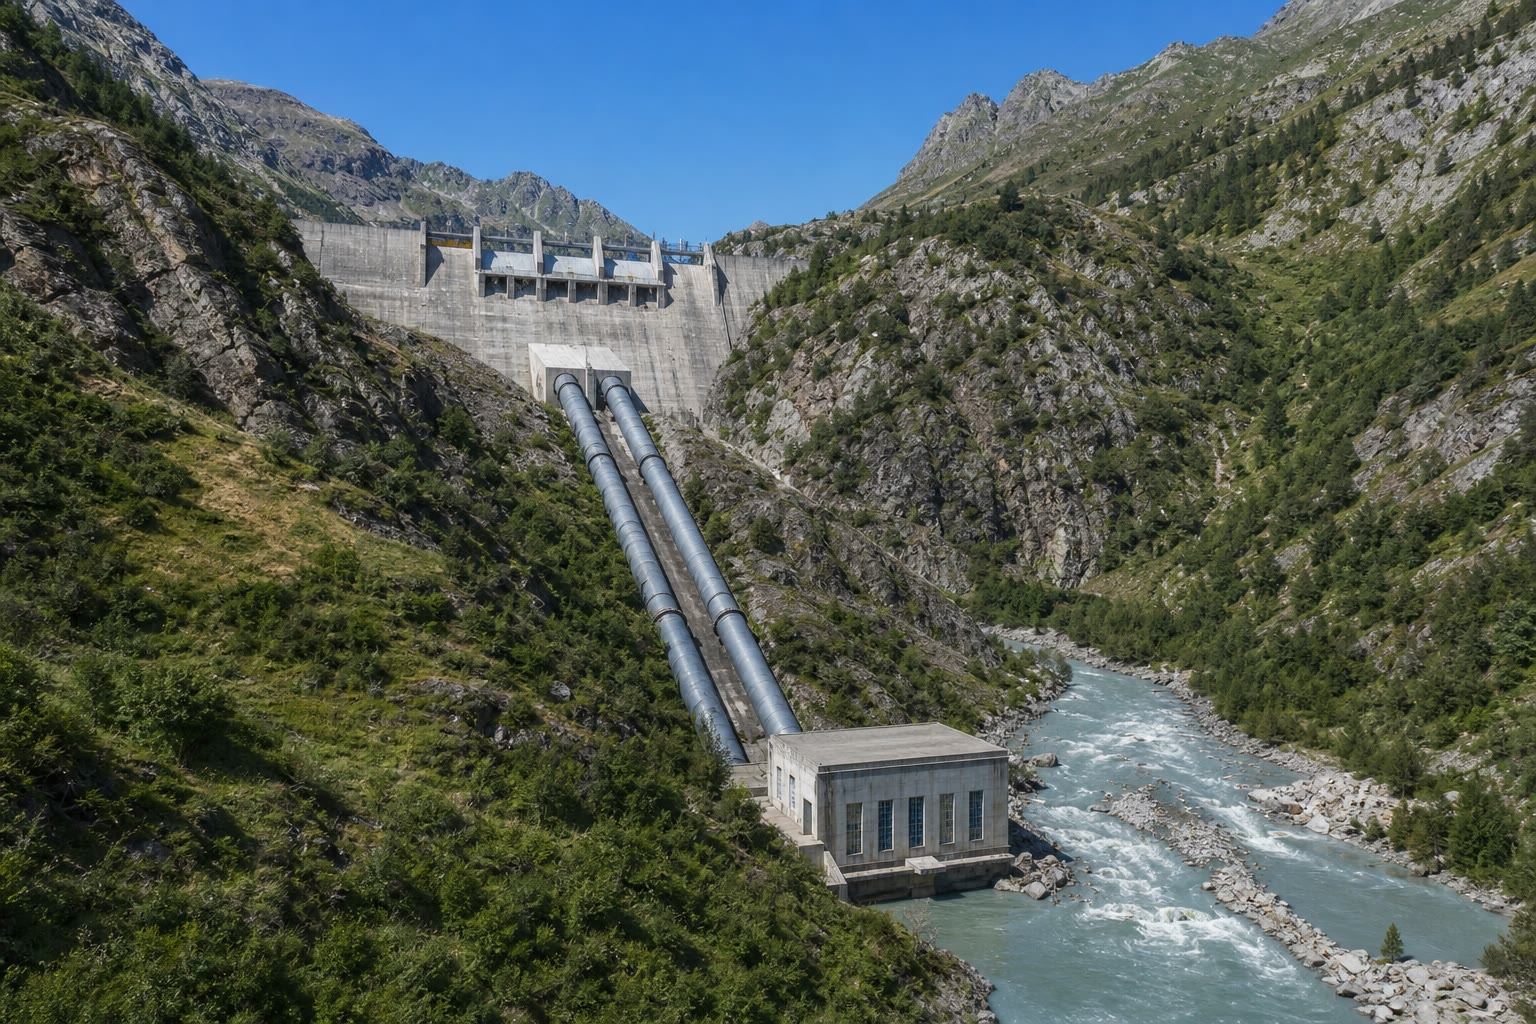
\includegraphics[width=0.58\linewidth]{images/book4/ai/b4-03-dam-penstock.jpg}

{\small 两条压力管将山区水库的水输送至涡轮机房：水头为两百米，由伯努利定理转化为每秒六十米的射流。}
\end{omfigure}

\section{问题：大坝、压力管与涡轮机}

\begin{problem}[{周末问题——水电站：从水库到射流的
压强、速率、功率、损失与
水锤}]
\label{pb:b2:euler-bernoulli:1}

水库在大坝后蓄水，水深 \qty{150}{m}；其自由面
高出涡轮机喷管 $H = \qty{200}{m}$。压力管（一根
钢管）直径为 $D = \qty{3.0}{m}$，长度为 $\ell = \qty{400}{m}$，
将设计流量 $D_V = \qty{60}{m^3/s}$ 输送至涡轮机房，
在那里，喷管将水转化为大气压强为 $P_0 =
\qty{1.0}{bar}$ 的自由射流，冲击佩尔顿轮的斗叶。$\rho =
\qty{1000}{kg/m^3}$，$g = \qty{9.81}{m/s^2}$；除非另有
说明，流体视为\omterm{def:b2:euler-bernoulli:perfect}{理想流体}。

\medskip
\noindent\textbf{第一部分——静止与设计流量。}
\begin{enumerate}
  \item 求大坝底部的压强，以及作用于大坝上
        宽 \qty{1}{m} 的竖直条带（自顶至底）的力。
  \item 涡轮机阀门关闭时，
        涡轮机房处压力管内的压强。
  \item 求设计流量下压力管内的速率，以及该处的\omterm{thm:b2:euler-bernoulli:bernoulli}{动压}；
        求压力管靠近涡轮机房一端（喷管之前）
        的压强，由水库表面应用伯努利方程求得。
  \item 求自由射流的速率；求喷管的截面与直径。
  \item 求射流携带的动能功率，证明其等于 $\rho gD_VH$，
        并计算其值。
  \item 求设计流量下压力管内所含水的质量与动能；
        求一个质点沿管道下行的渡越时间。
  \item 证明在设计流量下，水头 $H$ 由
        压力管底部的压强与水的动能分担，
        并说明喷管将前者转化为后者，
        求喷管之后的压强。
  \item \omterm{def:b2:euler-bernoulli:perfect}{理想流体}没有水头损失，实际流体则有：
        管道中的损失为 $\Delta P = \lambda(\ell/D)\,\tfrac12\rho v^2$，其中光滑钢管的 $\lambda
        \approx 0.015$。求以米水柱表示的水头损失，
        以及损失功率所占的比例。
  \item 工程师提议用 \qty{2}{m} 的压力管以节省钢材。重做
        第 7 题，并加以评论。
\end{enumerate}

\medskip
\noindent\textbf{第二部分——测量流量。}
压力管中装有文丘里管，喉部口径为 \qty{2.0}{m}。
\begin{enumerate}[resume]
  \item 求设计流量下喉部的速率，
        以及管道与喉部之间的压强降。
  \item 压强降由水银压差计读出（$\rho_{\text{Hg}} =
        \qty{13600}{kg/m^3}$）：求高度差。
  \item 证明流量与压差计读数的平方根成正比，
        并给出设计流量一半时的
        读数。
  \item 为何测压孔必须与管壁齐平，
        而不能伸入流体中？
  \item 因地形原因，管道的一段要越过
        一个顶点，该顶点\emph{高出}水库表面 \qty{6}{m}。求设计流量下该处的压强，
        会发生什么？设计者应当如何处理？
\end{enumerate}

\medskip
\noindent\textbf{第三部分——非定常工况。}
水库的表面积为 $A = \qty{2.0}{km^2}$。
\begin{enumerate}[resume]
  \item 设计流量下水库水位的下降速率，
        单位为厘米每小时。
  \item 涡轮机停机，喷管（第 4 题中的截面）
        对大气敞开，水库靠重力排水。写出
        质量平衡方程，并求水位 $h(t)$（准定常
        托里拆利流动）。
  \item 水位下降 \qty{10}{m} 所需的时间；
        与设计流量恒定时所需的时间作比较。
  \item 电站启动：压力管道已充满水，喷管
        于 $t = 0$ 时打开。取沿管道速度均匀，
        忽略喷管的几何形状，沿管道对\omterm{thm:b2:euler-bernoulli:euler}{欧拉方程}积分，
        得 $\ell\,\dd v/\dd t = gH - v^2/2$，求解之，
        并给出时间常数。
  \item 启动过程中，当 $v$ 为其终值的一半时，
        压力管道底部的压强为多少？
        并解释该压强与稳态值之差的符号。
\end{enumerate}

\medskip
\noindent\textbf{第四部分——关闭阀门。}
\begin{enumerate}[resume]
  \item 涡轮机处的阀门在 $\tau = \qty{10}{s}$ 内关闭；
        假设压力管道中的水做匀减速运动。利用沿管道的
        \omterm{thm:b2:euler-bernoulli:euler}{欧拉方程}，估算阀门处的超压（以巴为单位）。
  \item 若为快速关闭，水不能视为不可压缩：一压力波
        以 $c = \qty{1400}{m/s}$ 沿管道向上传播（钢管中水的声速——
        见\cref{ch:b2:sound-waves}），
        超压为 $\Delta P = \rho c\,\Delta v$（儒可夫斯基）。
        求设计流量下突然停止时的超压值，并与
        静压作比较。压力波往返水库需要多长时间，
        这对“快速”一词的含义说明了什么，
        即“快速”究竟指什么？
  \item 为保护压力管道，设置\emph{调压室}——一竖直敞口竖井，
        截面积 $A_s = \qty{100}{m^2}$——接于自水库来的水平隧洞
        （长 $L = \qty{2000}{m}$，截面积 $A =
        \qty{7.0}{m^2}$）与压力管道的汇合处。突然关闭后，
        隧洞中的水继续流动，竖井中水位
        $z$ 上升。写出隧洞与竖井之间的
        质量守恒方程。
  \item 沿隧洞对\omterm{thm:b2:euler-bernoulli:euler}{欧拉方程}积分（\omterm{def:b2:euler-bernoulli:perfect}{理想流体}），证明
        $z$ 满足 $\ddot z + \dfrac{gA}{LA_s}z = 0$，求其振动
        周期。
  \item 求从设计流量突然关闭后竖井中水位的最大上升量；
        （能量论证：隧洞中水的动能
        转化为竖井中水的势能）。
  \item 小结：列出本电站涉及的五种压强
        （大坝处静压、涡轮机处静压、管道中\omterm{thm:b2:euler-bernoulli:bernoulli}{动压}、水锤、
        涌浪），并给出各自对应的规律。
\end{enumerate}
\end{problem}
